Une fois le signal numérique reçu par l'ADC, il est important de passer ce signal dans un filtre numérique afin de ne conserver que les informations pertinentes (voir Fig. \ref{fig:filtrenumbloc}). Pour ce faire, nous avons dû faire face à différents choix afin de modéliser le filtre de la manière la plus efficace possible.

\begin{figure}[H]
    \centering
    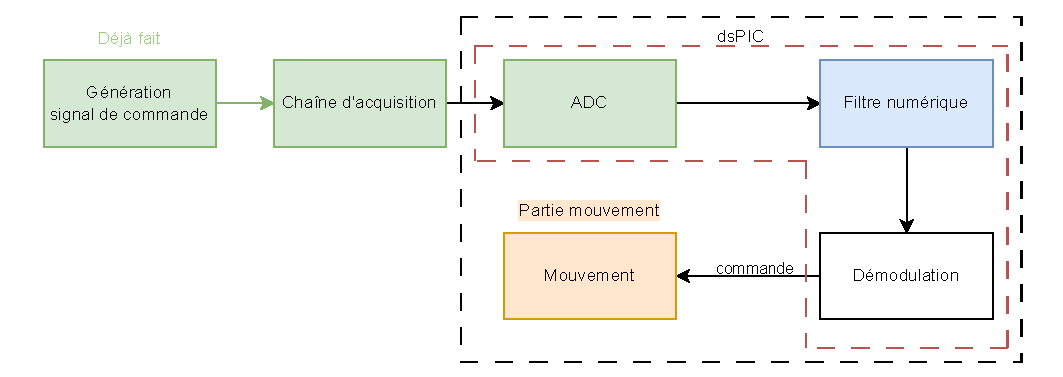
\includegraphics[scale=0.8]{pdffiles/filtrenumbloc.pdf}
    \caption{Schéma-bloc de la partie communication, focalisé sur le filtre numérique. La partie en rouge est détaillée sur la Figure \ref{fig:block_diagram}}
    \label{fig:filtrenumbloc}
\end{figure}

\begin{figure}[h]
    \centering
    \begin{tikzpicture}[node distance=2cm, auto]
        % ADC Block
        \node [block,fill=mygreen] (adc) {ADC};
        
        % Blocks for 900 Hz
        \node [block, right of=adc, node distance=3cm, fill=myblue] (filter1) {Filtrage (900 Hz)};
        \node [block, right of=filter1, node distance=3cm] (window1) {Fenêtre (900 Hz)};
        \node [block, right of=window1, node distance=3cm] (detector1) {Détecteur d'amplitude (900 Hz)};
        
        % Blocks for 1100 Hz
        \node [block, below of=filter1, node distance=2.5cm, fill=myblue] (filter2) {Filtrage (1100 Hz)};
        \node [block, right of=filter2, node distance=3cm] (window2) {Fenêtre (1100 Hz)};
        \node [block, right of=window2, node distance=3cm] (detector2) {Détecteur d'amplitude (1100 Hz)};
        
        % Demodulation Block
        \node [block, right of=detector1, node distance=4cm, text width=8em] (demod) {Démodulation\\ (FskDetector)};

        % Connecting lines for 900 Hz
        \path [line] (adc) -- (filter1);
        \path [line] (filter1) -- (window1);
        \path [line] (window1) -- (detector1);
        \path [line] (detector1) -- (demod);
        
        % Connecting lines for 1100 Hz
        \path [line] (adc) -- (filter2);
        \path [line] (filter2) -- (window2);
        \path [line] (window2) -- (detector2);
        \path [line] (detector2) -- (demod);
    \end{tikzpicture}
    \caption{Schéma-bloc détaillé entre l'ADC et la Démodulation, focalisé sur le filtre numérique}
    \label{fig:block_diagram}
\end{figure}

\subsection{Filtre FIR ou IIR}

\subsubsection{Filtres FIR}

Les filtres FIR sont caractérisés par une structure qui ne fait pas appel à la rétroaction. Leur sortie est calculée uniquement à partir de leur entrée et ils ont l'équation suivante:
\[
y[n] = \sum_{i=0}^{N} b_i x[n-i]
\]
où $b_i$ sont les coefficients du filtre, $x[n]$ est le signal d'entrée, et $N$ est l'ordre du filtre.

Les principaux avantages des filtres FIR sont leur bonne stabilité et la possibilité de réaliser une réponse en fréquence strictement linéaire. Cependant, pour atteindre des spécifications strictes de la bande de transition et de l'atténuation dans la bande d'arrêt, ils requièrent un ordre très élevé, ce qui est peu pratique dans le cadre de ce projet.

\subsubsection{Filtres IIR}

À l'opposé, les filtres IIR utilisent la rétroaction dans leur structure, ce qui les rend plus efficaces qu'un filtre FIR du même ordre pour obtenir une meilleure atténuation. L'équation générale d'un filtre IIR est:
\[
y[n] =  \sum_{j=0}^{N} b_j x[n-j] - \sum_{i=1}^{N} a_i y[n-i]
\]
où $a_i$ et $b_j$ sont les coefficients du filtre, et $N$ est l'ordre du filtre.

Les filtres IIR peuvent être instables si les pôles sont mal placés, mais une bonne conception permet d'éviter ces problèmes.

\subsubsection{Comparaison et Choix}

\textbf{Complexité computationnelle}

Le principal avantage des filtres IIR sur les FIR est leur faible ordre pour une atténuation donnée dans la bande d'arrêt, ce qui se traduit par moins de coefficients et donc moins d'opérations arithmétiques par échantillon traité. Ceci est particulièrement bénéfique dans les applications embarquées où la puissance de calcul et la mémoire sont limitées.

\textbf{Performance en Temps Réel}

La structure récursive des filtres IIR permet une implémentation plus efficace sur des processeurs simples, tels que le dsPIC utilisé pour le robot. Cette efficacité est très importante pour assurer une démodulation rapide et sans perte d'informations.

Le choix entre FIR et IIR dépend aussi des spécificités du système, notamment la tolérance aux phases non-linéaires et la nécessité d'une stabilité absolue. Pour notre robot, la légère phase non-linéaire introduite par un filtre IIR est un compromis acceptable pour bénéficier de sa faible complexité et de sa haute efficacité. Nous avons donc décidé de faire un filtre numérique IIR.

\subsection{Design du filtre numérique}
Pour concevoir les différents étages du filtre numérique, le code Python mis à notre disposition dans le cadre du projet est \textit{digitalFilterDesign.py}. Les filtres passe-bande ont été conçus selon les spécifications suivantes pour chaque fréquence centrale.

\subsubsection{Filtre Passe-Bande à 900 Hz}
\begin{itemize}
\item Fréquence d'échantillonnage : 16000 Hz
\item Fréquence centrale : 900 Hz
\item Largeur de la bande passante : 27 Hz
\item Gain minimum dans la bande passante : 0.9
\item Largeur de la bande bloquante : 63 Hz
\item Gain maximum dans la bande bloquante : 0.1
\end{itemize}

Les coefficients des étages du filtre sont les suivants :
\begin{align*}
    H_1(z) &= 0.001771 \frac{1+2z^{-1}+z^{-2}}{1-1.86370006z^{-1}+0.98824962z^{-2}} \\
    H_2(z) &= 0.001726 \frac{1+2z^{-1}+z^{-2}}{1-1.86719114z^{-1}+0.98840267z^{-2}} \\
    H_3(z) &= 0.023 \frac{1-2z^{-1}+z^{-2}}{1-1.86766577z^{-1}+0.99507105z^{-2}} \\
    H_4(z) &= 0.02283 \frac{1-2z^{-1}+z^{-2}}{1 -1.87591938z^{-1}+ 0.99522511z^{-2}}
\end{align*}
Le gain maximum des étages est 1.6757.

\begin{figure}[H]
    \centering
    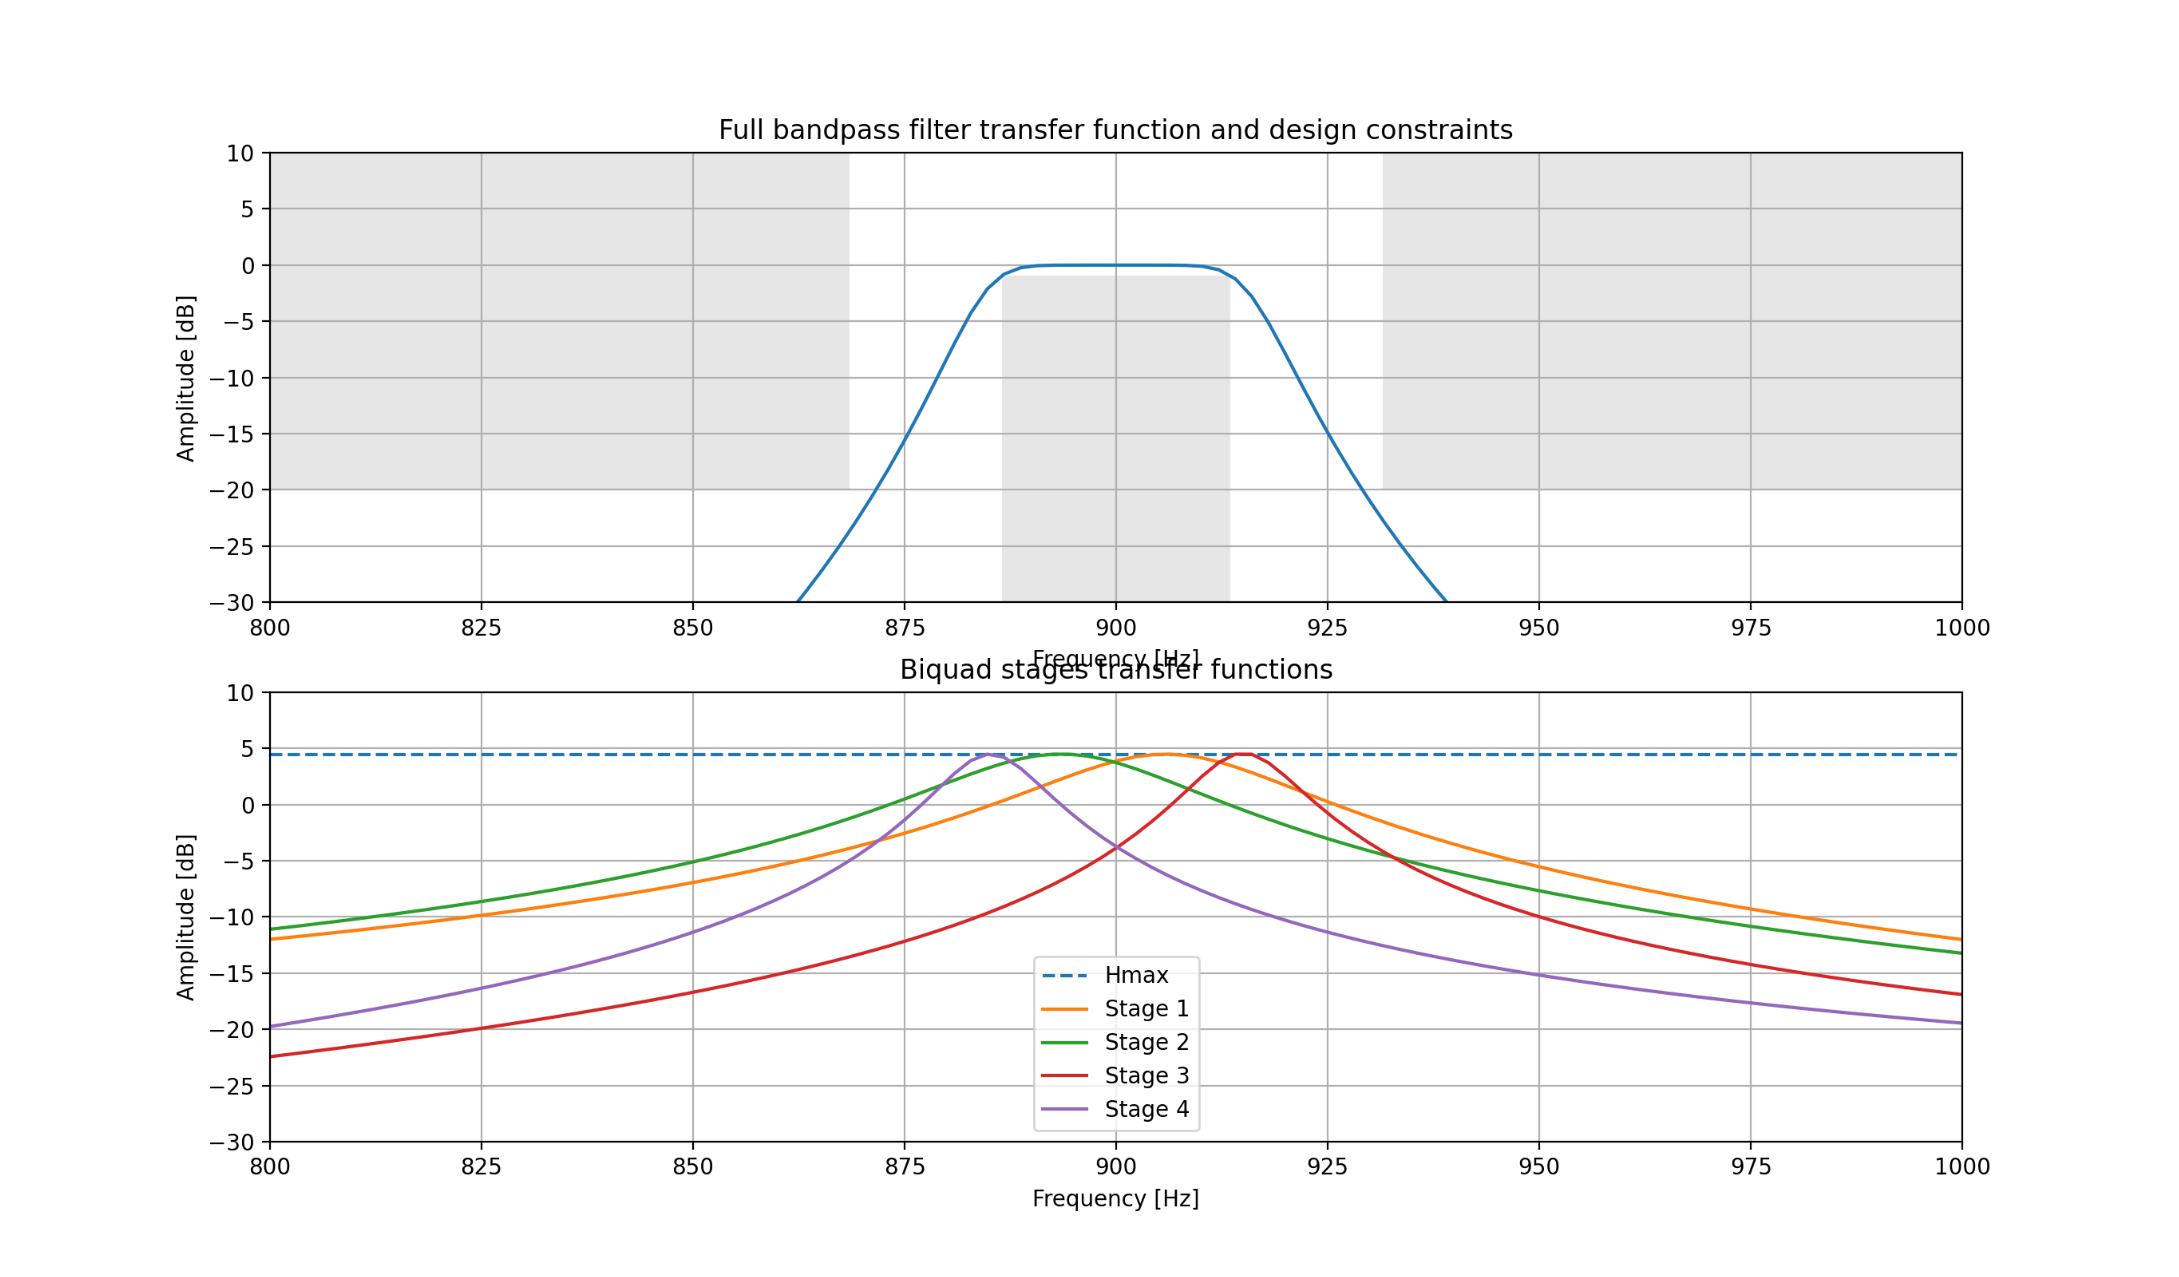
\includegraphics[width=0.7\textwidth]{Pictures/filtre iir 900.png}
    \caption{Filtre passe bande et des différents étages pour la fréquence centrale à 900Hz}
    \label{fig:enter-label}
\end{figure}

\subsubsection{Filtre Passe-Bande à 1100 Hz}
\begin{itemize}
    \item Fréquence d'échantillonnage: 16000 Hz
    \item Fréquence centrale: 1100 Hz
    \item Largeur de la bande passante: 33 Hz
    \item Gain minimum dans la bande passante: 0.9
    \item Largeur de la bande bloquante: 77 Hz
    \item Gain maximum dans la bande bloquante: 0.1
\end{itemize}

Les coefficients des étages du filtre sont les suivants:
\begin{align*}
    H_1(z) &= 0.00259 \frac{1+2z^{-1}+z^{-2}}{1-1.80592184z^{-1}+0.98584165z^{-2}} \\
    H_2(z) &= 0.002661 \frac{1+2z^{-1}+z^{-2}}{1-1.80081358z^{-1}+0.98565917z^{-2}} \\
    H_3(z) &= 0.02277 \frac{1-2z^{-1}+z^{-2}}{1-1.8047745z^{-1}+0.99398116z^{-2}} \\
    H_4(z) &= 0.02273 \frac{1-2z^{-1}+z^{-2}}{1-1.8169234z^{-1}+0.99416513z^{-2}}
\end{align*}
Le gain maximum des étages est 1.6796.
\begin{figure}[H]
    \centering
    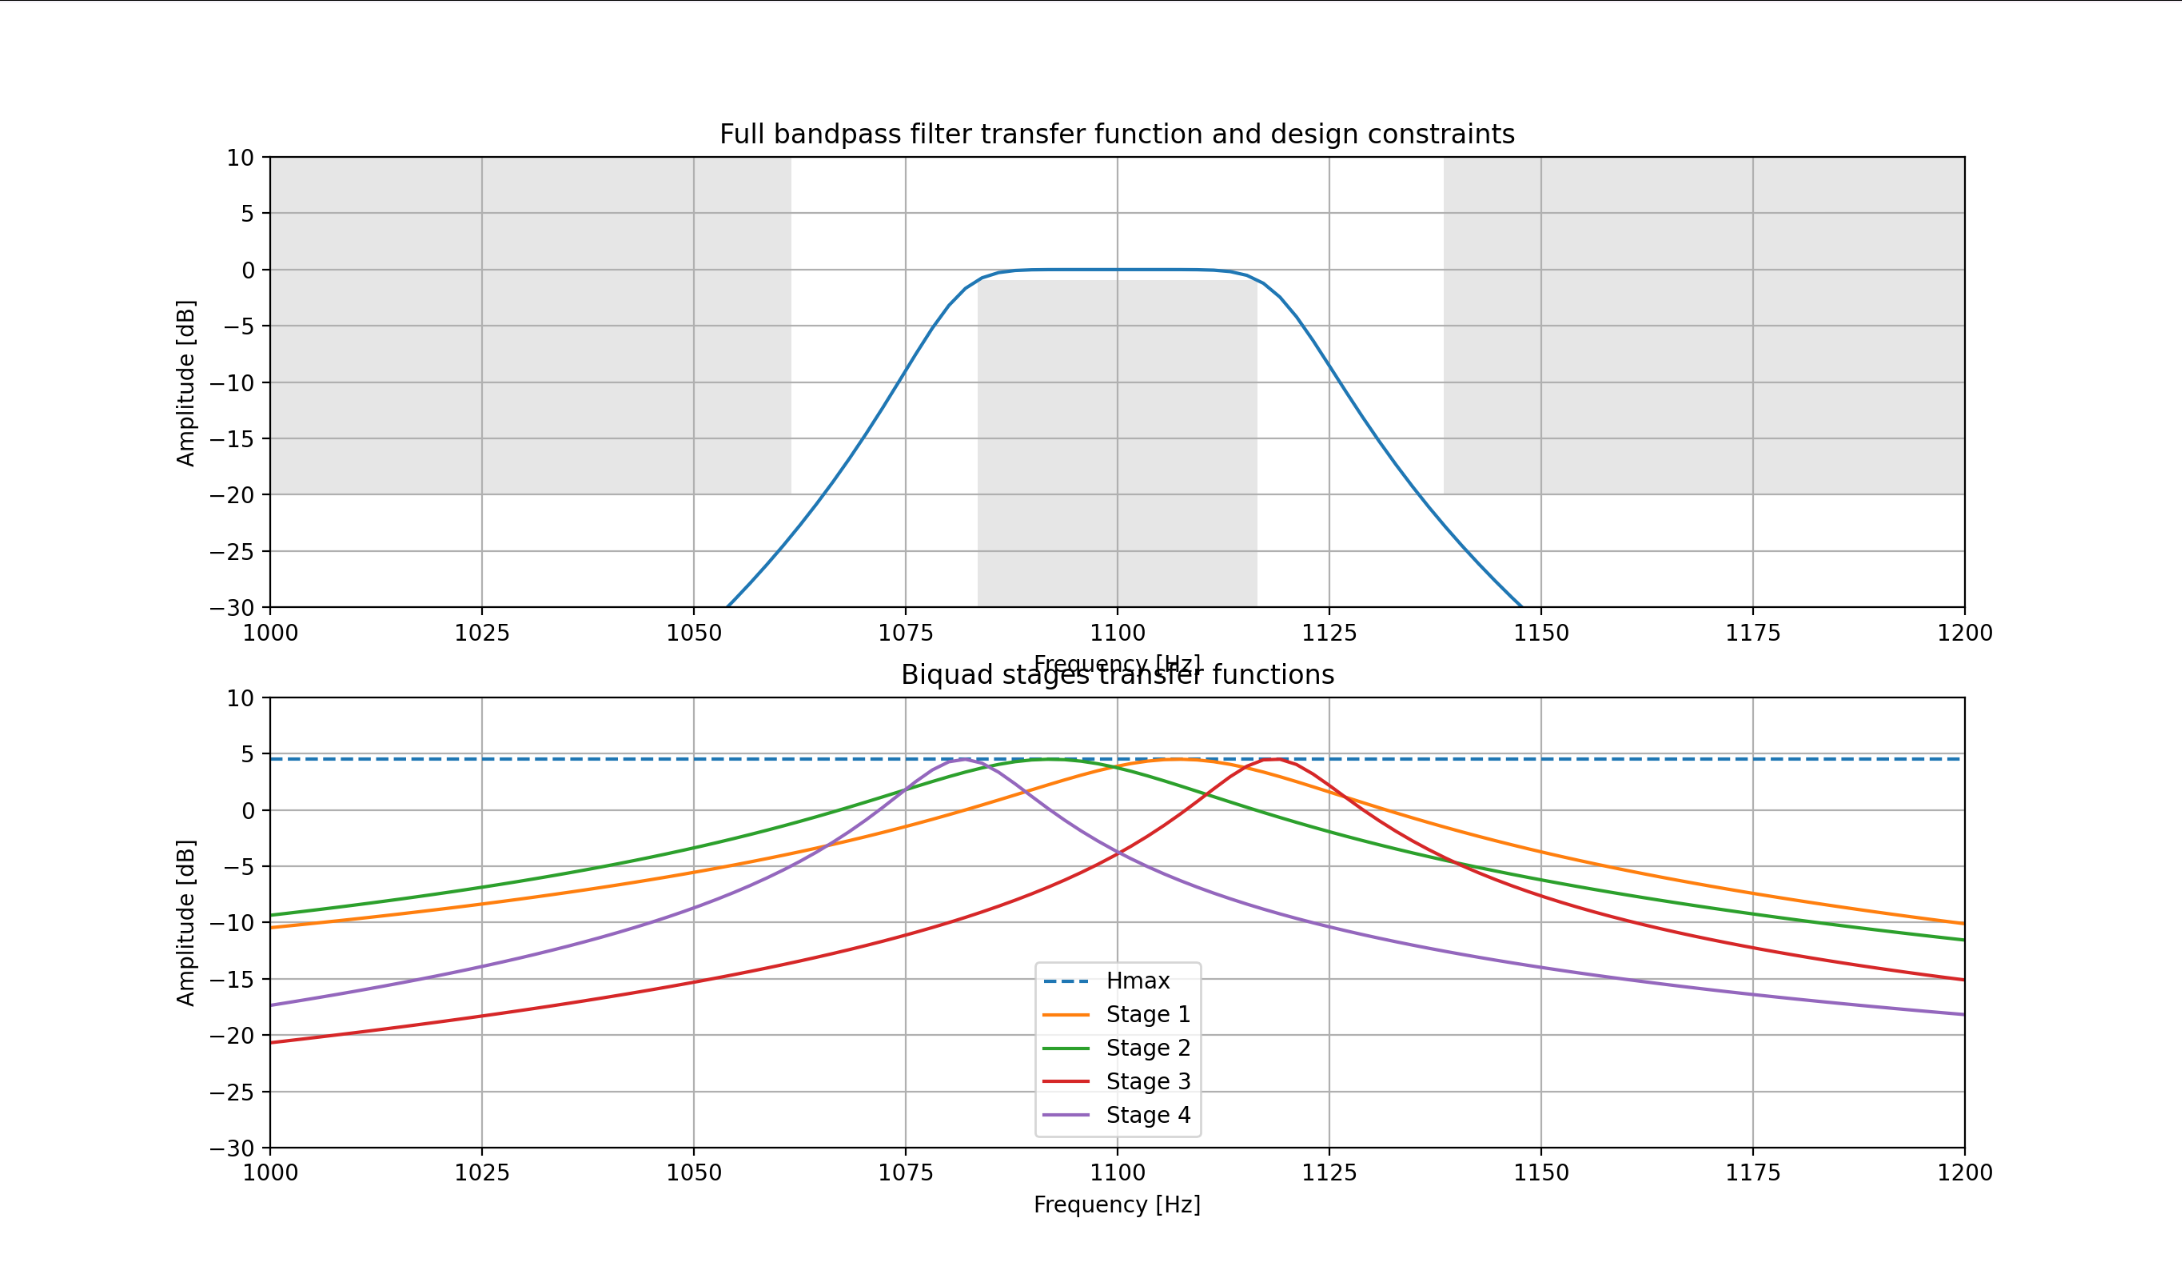
\includegraphics[width=0.7\textwidth]{Pictures/filtre iir 1100.png}
    \caption{Filtre passe bande et des différents étages pour la fréquence centrale à 1100Hz}
    \label{fig:enter-label}
\end{figure}



\input{Filtre num/Implémentation}
\section{Fenêtre Glissante et Seuil d'Amplitude}
\begin{figure}[h]
    \centering
    \begin{tikzpicture}[node distance=2cm, auto]
        % ADC Block
        \node [block,fill=mygreen] (adc) {ADC};
        
        % Blocks for 900 Hz
        \node [block, right of=adc, node distance=3cm, fill=mygreen] (filter1) {Filtrage (900 Hz)};
        \node [block, right of=filter1, node distance=3cm,fill=myblue] (window1) {Fenêtre (900 Hz)};
        \node [block, right of=window1, node distance=3cm,fill=myblue] (detector1) {Détecteur d'amplitude (900 Hz)};
        
        % Blocks for 1100 Hz
        \node [block, below of=filter1, node distance=2.5cm,fill=mygreen] (filter2) {Filtrage (1100 Hz)};
        \node [block, right of=filter2, node distance=3cm,fill=myblue] (window2) {Fenêtre (1100 Hz)};
        \node [block, right of=window2, node distance=3cm,fill=myblue] (detector2) {Détecteur d'amplitude (1100 Hz)};
        
        % Demodulation Block
        \node [block, right of=detector1, node distance=4cm, text width=8em] (demod) {Démodulation\\ (FskDetector)};

        % Connecting lines for 900 Hz
        \path [line] (adc) -- (filter1);
        \path [line] (filter1) -- (window1);
        \path [line] (window1) -- (detector1);
        \path [line] (detector1) -- (demod);
        
        % Connecting lines for 1100 Hz
        \path [line] (adc) -- (filter2);
        \path [line] (filter2) -- (window2);
        \path [line] (window2) -- (detector2);
        \path [line] (detector2) -- (demod);
    \end{tikzpicture}
    \caption{Schéma-bloc détaillé entre l'ADC et la Démodulation, focus sur la fenêtre et la détection d'amplitude}
    \label{fig:block_diagram_fe}
\end{figure}
\subsection{Fenêtre Glissante}
\label{fenetre_glissante}
Pour implémenter la démodulation du signal, nous avons implémenter une fenêtre glissante permettant de choisir la plus grande valeur parmi les échantillons dans la fenêtre. La fréquence d'échantillonnage étant de 16 kHz, il a fallu faire une fenêtre glissante sur $\frac{16000 \text{ Hz}}{900 \text{ Hz}} \approx 17$ échantillons et sur $\frac{16000 \text{ Hz}}{1100 \text{ Hz}} \approx 15$ échantillons. Il est acceptable de considérer une fenêtre glissante identique pour les deux fréquences prenant en compte 16 échantillons. Il est important de considérer que désormais, à la sortie de ce bloc, nous ne travaillons plus à 16 kHz mais bien à 1 kHz, étant donné que la fenêtre glissante ne renvoie que le plus grand échantillon parmi 16. 

\subsubsection{Implementation de la Fenêtre Glissante}
Une fois que les échantillons ont été filtrés, un maximum est déterminé dans une fenêtre glissante de 16 échantillons. Pour chaque échantillon traité, s'il s'agit du premier échantillon de la fenêtre, il est initialisé comme maximum. Pour les échantillons suivants, une comparaison est faite pour déterminer si l'échantillon filtré courant est supérieur au maximum actuel. Si c'est le cas, il devient le nouveau maximum.
\subsection{Seuil d'Amplitude}
Le plus grand échantillon à la sortie de la fenêtre glissante est ensuite comparé à un seuil d'amplitude. Ce seuil est choisi en fonction des valeurs des filtres obtenues lors de la simulation du filtre numérique. Pour rappel, les amplitudes maximales obtenues en virgule flottante sur les graphes pour 900 Hz et 1100 Hz étaient respectivement de 3 et 0.75 (\ref{res_filtre_num}).

Dans le code, la sortie du filtre est en virgule fixe. Par conséquent, des seuils de 500 et de 150 ont été choisis pour les amplitudes à 900 Hz et 1100 Hz respectivement. Ces valeurs ont été déterminées à partir de différents tests visant à ajuster précisément les seuils. L'objectif était de trouver un équilibre entre des seuils suffisamment élevés pour éviter que le bruit ne soit interprété comme un signal, mais pas trop élevés afin de ne pas manquer les véritables signaux. Ainsi, les seuils de 500 pour 900 Hz et de 150 pour 1100 Hz garantissent une détection fiable et précise des signaux. La fonction du seuil d'amplitude renvoie 0 si l'amplitude est inférieur au seuil et 1 pour le cas inverse.




\input{Filtre num/Démodulation}
\section{Conclusion du traitement des signaux audio}

Les sections 3.1 à 3.5 de notre projet montrent l'importance d'un traitement du signal  pour assurer le bon fonctionnement de notre robot. Nous avons dimensionné une chaîne d'acquisition qui remplit le cahier des charges. Ensuite, la conversion analogique-numérique (ADC) a été configurée pour permettre une démodulation rapide sans surcharger le CPU. En choisissant des filtres IIR, nous avons pu obtenir une atténuation efficace avec un ordre minimal, facilitant une implémentation rapide et précise. L'utilisation d'une fenêtre glissante de 16 échantillons pour sélectionner le maximum a permis de réduire la fréquence d'échantillonnage effective, tandis que les seuils d'amplitude ajustés empêchent les faux positifs tout en assurant la détection correcte des signaux. La fonction \texttt{fskDetector} analyse les bits 1 ou 0 des deux fréquences centrales à la sortie du seuil d'amplitude pour déterminer l'état du signal et créer une trame de bits, ce qui permet au robot de savoir quelle action exécuter. Il a fallu que toutes ces étapes soient réalisées en moins de 62.5 $\mu$s pour s'assurer de ne pas perdre des informations du signal.

